\begin{enumerate}[label=\thesection.\arabic*.,ref=\thesection.\theenumi]
\numberwithin{equation}{enumi}
\item Plot the polar plot of 
\begin{align}
G(s) = \frac{1}{(s^2)(s+1)(s+2)}. 
\end{align}

\solution
For polar plot we have to plot magnitude of $G(s)$ versus its phase
by varying $\omega$ from 0 to $\infty$.

First substitute, 
\begin{align}
    s = j\omega
\end{align}
Now the magnitude will be
\begin{align}
|G(j\omega)| = \frac{1}{(\omega^2)(\sqrt{1 + \omega^2})(\sqrt{1+4\omega^2})} 
\end{align}

\begin{figure}[!h]
  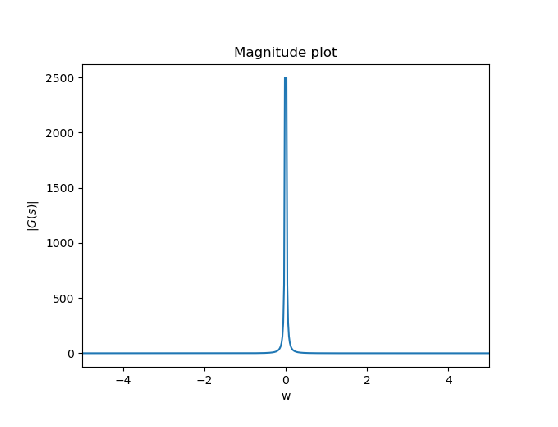
\includegraphics[width=\columnwidth]{magnitude.eps}
\end{figure}

Similarly phase $\phi$ can be determined by,

\begin{align}
  \phi = - \tan^{-1}(0) - \tan^{-1}(\omega) - \tan{-1}(2\omega)
\end{align}
The phase of first term is $\pi$ or can be $-\pi$ since it is a negative real number.
\begin{align}
    \implies \phi = 180\degree - \tan^{-1}(\omega) - \tan{-1}(2\omega)
\end{align}

Now we have to sweep $\omega$ from 0 to $\infty$.

So at $\omega = 0$,
\begin{align}
    |G| \xrightarrow{0} \infty 
\end{align}
And phase,

\begin{align}
    \angle {G} = 180 \degree
\end{align}

At $\omega = \infty$
\begin{align}
    |G| \xrightarrow{\infty} 0
\end{align}
 And phase,
\begin{align}
    \angle {G} = 0 \degree
\end{align}

Thus the polar plot looks like, 
\newline
\newline
\begin{figure}[!h]
  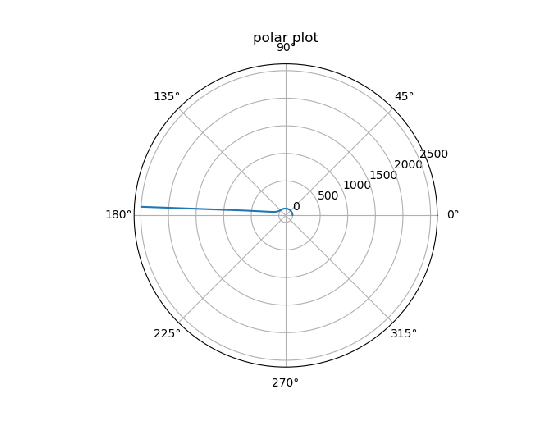
\includegraphics[width=\columnwidth]{polarplot.eps}
\end{figure}

To take a closer look at how phase is changing in smaller ranges of $\omega$.
\begin{figure}[!h]
  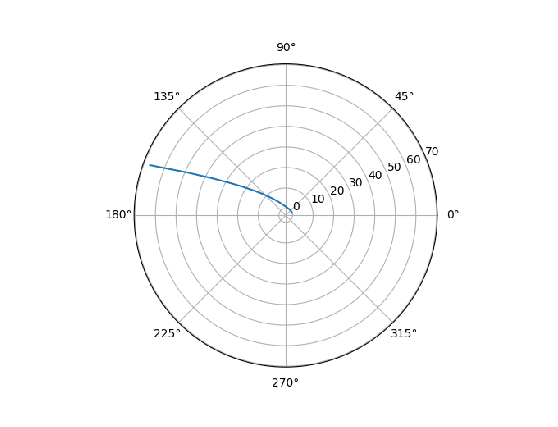
\includegraphics[width=\columnwidth]{polar_plot2.eps}
\end{figure}



\end{enumerate}
